\documentclass{sigchi}

% Use this command to override the default ACM copyright statement
% (e.g. for preprints).  Consult the conference website for the
% camera-ready copyright statement.


%% EXAMPLE BEGIN -- HOW TO OVERRIDE THE DEFAULT COPYRIGHT STRIP -- (July 22, 2013 - Paul Baumann)
% \toappear{Permission to make digital or hard copies of all or part of this work for personal or classroom use is      granted without fee provided that copies are not made or distributed for profit or commercial advantage and that copies bear this notice and the full citation on the first page. Copyrights for components of this work owned by others than ACM must be honored. Abstracting with credit is permitted. To copy otherwise, or republish, to post on servers or to redistribute to lists, requires prior specific permission and/or a fee. Request permissions from permissions@acm.org. \\
% {\emph{CHI'14}}, April 26--May 1, 2014, Toronto, Canada. \\
% Copyright \copyright~2014 ACM ISBN/14/04...\$15.00. \\
% DOI string from ACM form confirmation}
%% EXAMPLE END -- HOW TO OVERRIDE THE DEFAULT COPYRIGHT STRIP -- (July 22, 2013 - Paul Baumann)


% Arabic page numbers for submission.  Remove this line to eliminate
% page numbers for the camera ready copy 

%\pagenumbering{arabic}

% Load basic packages
\usepackage{balance}  % to better equalize the last page
\usepackage{graphics} % for EPS, load graphicx instead 
%\usepackage[T1]{fontenc}
\usepackage{txfonts}
\usepackage{times}    % comment if you want LaTeX's default font
\usepackage[pdftex]{hyperref}
% \usepackage{url}      % llt: nicely formatted URLs
\usepackage{color}
\usepackage{textcomp}
\usepackage{booktabs}
\usepackage{ccicons}
\usepackage{todonotes}

% llt: Define a global style for URLs, rather that the default one
\makeatletter
\def\url@leostyle{%
  \@ifundefined{selectfont}{\def\UrlFont{\sf}}{\def\UrlFont{\small\bf\ttfamily}}}
\makeatother
\urlstyle{leo}

% To make various LaTeX processors do the right thing with page size.
\def\pprw{8.5in}
\def\pprh{11in}
\special{papersize=\pprw,\pprh}
\setlength{\paperwidth}{\pprw}
\setlength{\paperheight}{\pprh}
\setlength{\pdfpagewidth}{\pprw}
\setlength{\pdfpageheight}{\pprh}

% Make sure hyperref comes last of your loaded packages, to give it a
% fighting chance of not being over-written, since its job is to
% redefine many LaTeX commands.
\definecolor{linkColor}{RGB}{6,125,233}
\hypersetup{%
  pdftitle={SimpleSpeech: Simplified Audio Production in Asynchronous Voice-Based Discussions},
  pdfauthor={LaTeX},
  pdfkeywords={SIGCHI, proceedings, archival format},
  bookmarksnumbered,
  pdfstartview={FitH},
  colorlinks,
  citecolor=black,
  filecolor=black,
  linkcolor=black,
  urlcolor=linkColor,
  breaklinks=true,
}

% create a shortcut to typeset table headings
% \newcommand\tabhead[1]{\small\textbf{#1}}
\newcommand*{\red}{\textcolor{red}}

% End of preamble. Here it comes the document.
\begin{document}

\title{Simplified Audio Production in Asynchronous \\ Voice-Based Discussions}

\numberofauthors{1}
\author{%
  \alignauthor{(Anonymized)\\
  }
}

\maketitle

\begin{abstract}
  % Added a place-holder abstract, just so we have something to work
  % from
%  We present a novice-friendly system for construction of
%  high-quality audio narration. Unedited audio is often cumbersome --
%  as evidenced by the move from voicemail to text-based messaging
%  formats. However, text loses a lot of tone and
%  personality. Professionally produced voice narration is a pleasure
%  to listen to, but has traditionally been prohibitive for novices to
%  create. We present a system which uses automatic speech recognition
%  to convert waveforms into a human-friendly representation for
%  editing. Users can easily delete text, re-record audio segments, as
%  well as adjust timing. We have both qualitative and quantitative
%  results that the system results in a good user experience for novice
%  audio producers, and allows for the creation of high-quality audio
%  narration. We intend to apply the system to student-created content
%  in learning-at-scale settings.
Asynchronous audio communication (AAC) adds nuance and expressivity to virtual discussions, but its one-shot nature tends to discourage collaborators from utilizing it.
However, a text-based interface makes voice editing much easier, especially with recent advancements enabling live, time-aligned speech transcription.
We introduce SimpleSpeech, an easy-to-use voice production platform that takes advantage of real-time speech recognition. 
The system supports novel lightweight tools for inserting content, adjusting pauses, and correcting transcript errors.
Qualitative and quantitative results suggest that novice audio producers, such as high school students, experience greater success and decreased workload when using SimpleSpeech to produce audio messages than without editing.
The linguistic formality of voice comments was also studied, and found to form a middle ground between oral and written communication media.
When applied to appropriate contexts such as online learning at-scale, SimpleSpeech could serve the crucial purpose of lowering the barrier to engage in audio-based collaborative environments.
\end{abstract}

\keywords{Speech editing; transcription-based editing; asynchronous audio communication.}

\category{H.5.2.}{User Interface: Voice I/O}{}{}


\section{Introduction}

Asynchronous audio communication (AAC) is rapidly becoming available to mass audiences through social platforms such as WhatsApp, iMessage, and Facebook. 
While text is still by far the most prevalent mode of communication on the Internet, audio is desirable in many situations because it allows users to deliver more expressive, nuanced messages than text.

AAC holds considerable potential for improving collaboration in education and business as well. 
For instance, audio messages have been favorably used to disseminate feedback on assignments in online courses \cite{ice,oomen}. 
On the other hand, voice communication is much less prevalent in business environments now that voicemail, a paradigm that is generally regarded as ``onerous'' and ``laborious'' \cite{whittaker}, is on the decline. 
According to Grudin \cite{grudin}, the primary reason for the failure of voicemail is an inherent imbalance of workload between speaker and listener: message creators can speak more quickly than they can type, but recipients cannot listen as fast as they can read. 
Perhaps for this reason, email continues to predominate over voice messages in corporate communication despite the diminished individuality and, more critically, the higher risk of miscommunication in textual media \cite{byron}.

Despite these difficulties, AAC is undoubtedly superior to text for certain applications. 
For instance, audio messages can be used as annotations on virtual documents, enabling the user to process comments aurally without visual distraction \cite{yoon}.
Another area of benefit is in online education, where voice communication has been shown to improve student-student and student-instructor engagement as well as a sense of the instructor's social presence \cite{oomen,tu}. 
When applying AAC to online education, however, many students may have trouble articulating their ideas vocally.
This problem affects students even in physical classrooms and could prevent these learners from participating in online oral discussions.
The goal of AAC platforms in such situations, then, is not only to improve efficiency for consumers, but also to compensate for the linearity and immutability of audio on the production side.

Our solution is to provide lightweight, easy-to-use editing tools based on automatic speech recognition (ASR)-generated transcripts.
Prior studies have utilized transcription as a proxy for editing audio, but have been limited by the quality of ASR algorithms

We designed and developed a user-friendly audio production tool, which we call SimpleSpeech, and applied it to the scenario of discussion on an online forum. 
The mental workload experienced by high school students recording voice messages was shown to be significantly decreased with editing functionality, indicating that SimpleSpeech is a valuable enhancement to online audio communication platforms.
In addition, some linguistic characteristics of messages created using AAC are discussed with comparison to other forms of computer-mediated communication, leading to new considerations and insights on optimal applications of this technology.

\section{Related Work}

The linear, sequential nature of voice communication not only precludes skimming and navigation capabilities \cite{grudin}, but can also hamper the speech \emph{production} process. 
Voice production is a temporarily linear process which demands that the speaker thinks and speaks simultaneously \cite{marriott2002, yoon:2015}.
Therefore, cognitive load arises from the fact that one has to keep speaking to prevent undesirable long pauses. 
In addition, mistakes in recorded speech are harder to revise than textual typos, mainly due to the lack of lightweight voice editing software \cite{marriott2002}.  
Building on the qualitative implications of these previous works, our study presents a quantitative measure about how such burdens are reduced when the voice production system includes lightweight editing features.

Because lower-level audio waveform editing is an onerous task, speech manipulation tools have been developed that present audio in semantically meaningful higher-level chunks, such as words and phrases.
Acoustic detection of the presence of speech provides simple, discretized visual guidance so that users can edit or index the speech recording \cite{ades1986, hindus:1992}; on the other hand, a pure acoustic approach has limited recognition granularity. % I'm actually not sure what you're saying here. Is the part after the semicolon a compare-contrast or describing the limits of the first part?
Time-aligned automatic speech recognition (ASR) has now become a popular tool to achieve the word-level structuring of speech \cite{Schmandt81, Wilcox:1992}. 
Compared with acoustic structuring, ASR presents semantic information at higher resolution, but has also suffered from high computational load and delay. 
However, recent technical developments have made ASR faster and more accurate, and we take full benefit of this real-time transcription capability.

Since speech transcription elicits the contents of the recording, researchers have utilized it to assist in visual skimming and navigation. 
MedSpeak \cite{Lai:1997} and SCANMail \cite{whittaker} are well recognized as precursors of such systems that use time-alignment data of the transcript for indexing audio. 
Since transcription errors tend to obstruct visual comprehension, Vemuri et al. suggested a novel visualization of the transcript that adjusts transcription brightness to the word's ASR confidence score \cite{Vemuri:2004}. 

On the production side, there have been several systems that use a time-aligned transcript for editing audio \cite{rubin,whittaker_semantic,yoon} or video \cite{Berthouzoz:2012,casares}. 
Among them, Whittaker and Rubin's editing system leveraged users' familiarity with text-editing interfaces to adopt audio editing within that paradigm. 
Since we targeted non-professional users, our interface also took the text-like approach, but emphasizing a \emph{live} production process and going beyond editing already-transcribed speech. 

Just as with listeners, ASR errors can be detrimental for understanding and skimming audio contents during editing \cite{halverson1999beauty}. 
In the MedSpeak interface, Lai et al. provided a separate graphical window for fixing transcription errors \cite{Lai:1997}. 
In a speech production system like SimpleSpeech, though, users could easily get lost between the audio editing and transcription correction modes, so we chose to guide the user's attention through these modes via the movement of the editing caret into a quasi-modal interface.

Pauses in speech deliver nuanced meaning such as hesitation or emphasis, so easy and powerful manipulation of pause duration is important. 
A system called SpeechSkimmer automatically condenses pauses for fast auditory skimming \cite{arons:1993}. 
Other previous systems supported pause editing via a designated button \cite{Berthouzoz:2012} or specialized tags \cite{rubin}. 
Rubin et al.'s system used the period key as a shortcut to insert pause tags, but the duration of the gap was preset and required the use of a separate menu. 
Our approach is based on a traditional text editor, where users adjust lengths of pauses by adding and deleting spaces with the spacer bar and delete keys. The length of the pause corresponds to the number of spaces.

Perhaps most importantly, studies of the mental and linguistic effects of AAC discourse are limited despite the variety of AAC system designs discussed above.
Those studies that exist are focused on the larger category of computer-mediated communication (CMC), which is dominated by textual media such as SMS, email, or Facebook posts.
For example, Kiesler, Siegel, and McGuire \cite{kiesler} found more equalized group participation and more uninhibited expression of opinions in synchronous text-based CMC than in face-to-face discussions.
Asynchronous CMC, similar to a discussion board, induces more prosocial behavior and, in fact, more informal communication styles over time than face-to-face \cite{walther}.
On the other hand, formality and politeness in emails has been shown to increase as the social distance, status gap, and importance of a request increase \cite{cho}.
How these findings about textual media relate to spoken modes of CMC has not been heavily investigated, however.



\section{Designing SimpleSpeech}

Building on the capabilities developed in these prior studies, SimpleSpeech is a web-based application for recording and editing short voice messages in a discussion setting (see Fig. \ref{fig:overview_shot}).
The design of SimpleSpeech is largely inspired by the transcription-based speech editing systems developed by Rubin \cite{rubin}, Yoon \cite{yoon}, and Whittaker \cite{whittaker_semantic}, which also use ASR transcription as a semantic and visual proxy for audio.
In addition, some slight conceptual modifications were necessary to suit the ``live'' editing paradigm, in which the user records and edits spoken comments in a unified workflow.

We followed an iterative procedure to progressively improve the design and interactions of SimpleSpeech.
After building an initial prototype of the application, an informal pilot test was conducted with 5 participants (4 female, 1 male). 
Each user was given a brief introduction to the software and shown how to use the basic features, then given the scenario of creating an audio response to a written claim on an online forum. 
(The prompts used in the tests were adapted from the GRE Pool of Issue Topics.)
The user feedback helped us improve the capabilities of SimpleSpeech, including the following modifications:

\begin{itemize}
	\item \emph{Pause manipulation}. An important finding in the pilot study was the importance of being able to introduce and adjust pauses between words, not just to remove them.
	These gaps in the audio help make natural-sounding cuts between audio clips as well as to punctuate claims (e.g., the end of a sentence). 
	The original system only allowed the user to delete pauses, so we added a spacebar action to insert a fragment of silence from the original audio resource into the rendered message or to extend length of an existing pause token on which the cursor is prompting.
	\item \emph{Live insertion}. Users often misspoke a word or phrase in the middle of a message.
	Since re-recording the entire message was a large burden, a partial deletion and re-recording capability was required.
	Our interface maintains the text-based principle that the cursor position uniformly indicates the focus of editing.
	Therefore, in SimpleSpeech, clicking the Record button naturally inserts a new stream into the existing audio at the point corresponding to the cursor position.
	\item \emph{Quasi-modal transcription editing}. In consideration of the recipient, the pilot testers wanted to correct ASR errors.
	However, we found that our versatile text-like audio editing interface would confuse the user between the audio-editing mode for revising speech and text-editing mode for correcting mistranscriptions.
	This led us to design a small, separate quasi-modal editing box (see Fig. \ref{fig:transcription}) that pops up during transcription editing.
	The movement of the cursor to the modal box clearly indicates that the system is in a separate text-editing mode, accessed by pressing the Return key.
\end{itemize}



\begin{figure}
	\centering
	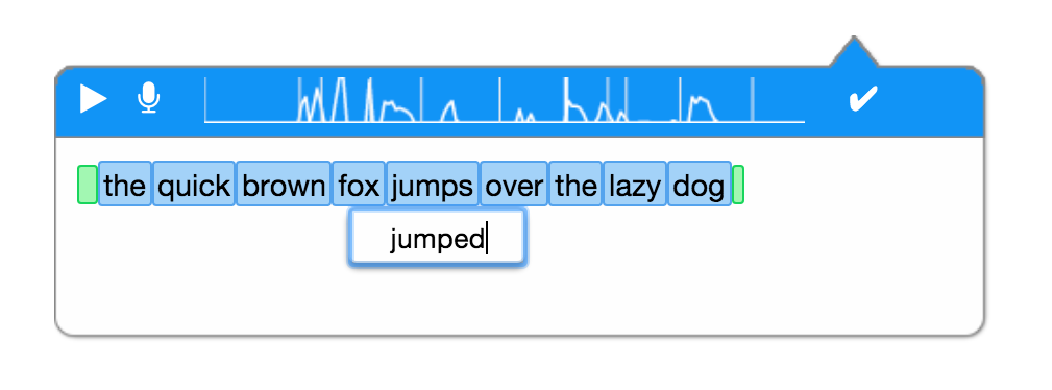
\includegraphics[width=\columnwidth,keepaspectratio]{figures/transcription_edit}
	\caption{To keep the user interface from becoming cluttered with secondary functionality, the transcription editing feature was implemented as a modal interaction. The pop-up box shown above ``opens'' the selected tokens for text editing in a separate control element, thus notifying the user that he or she is no longer directly editing the audio.}
	\label{fig:transcription}
\end{figure}


Our text-based approach to speech editing requires a reliable transcription as well as time intervals corresponding to each word.
Both of these requirements are fulfilled by the IBM Watson Developer Cloud speech-to-text transcription service, which is reported to have a word error rate of 10.4\% \cite{soltau:2014}.

\section{Qualitative Evaluation}

The interaction paradigm of SimpleSpeech was tested in a qualitative assessment to determine (1) the practicability of a lightweight text-based audio editor, (2) the effects of minor transcription errors on audio consumption and production, and (3) the implications of being able to edit audio in an asynchronous online discussion.

Participants were introduced to the functionality of the system, then given two untimed tasks. 
First, to simulate an asynchronous audio discussion, the test users were asked to listen to an audio comment left by the previous tester and create an original audio response. 
Next, they received a different, textual prompt and created an audio comment which would be consumed by the next user. 
In both cases the user was asked to edit his or her recording to be polished and clear.
The participants were interviewed at the end of the test; these interviews were transcribed, conversational elements filtered out, and the remaining sentences analyzed via open coding followed by flat coding. Cohen's $\kappa$ was .78, indicating high reliability between the two coders.

The sample for the study consisted of 9 test subjects (4 male, 5 female, mean age 21.6 yrs; henceforth denoted $P_1, P_2, \ldots, P_9$). 
All participants were native English speakers. 
Two individuals, $P_2$ and $P_3$, were professional media editors who provided technical feedback and a comparison to pure audio editing; the remainder were interns and high school students.

\subsection{Results}
The coding process resulted in the following themes identified from the user feedback:

\emph{The text-based editing paradigm provides sufficient control to render waveform manipulation unnecessary.}
Most non-professional users felt SimpleSpeech gave them ``plenty of control'' over the editing process ($P_4,\,P_5,\,P_6,\,P_8$). 
The professional editors did note that most people in their field would not find SimpleSpeech adequate for their needs; but, as $P_2$ conceded, the intended market users ``don't have to play with the settings which is why they don't use a professional audio editor.''
Most participants characterized the editing experience as being a text-focused one, suggesting that the translation to text was in fact a useful proxy for editing audio. 
The text modality was described as ``more accessible, more doable'' than pure waveform editing, which could be ``scary for people who don't do video stuff'' ($P_3,\,P_7$). 

\emph{The primary use of lightweight voice editing is to make fine-grained rather than large-scale adjustments.}
The most commonly-used manipulation during the qualitative study was the removal of disfluencies ($P_1,\,P_2,\,P_4,\,P_5,\,P_7$), followed by pause deletion ($P_2,\,P_3,\,P_5,\,P_6,\,P_8$). 
Only $P_1$ and $P_8$ edited large chunks of audio by deleting or rerecording, and $P_8$ reported doing so only to improve the smoothness of a smaller change in a sentence.
Perhaps because SimpleSpeech was presented as a tool to be briefly used to ``clean up'' recordings, participants focused on removing the ``embarrassing'' and ``awkward'' sounds ($P_1,\,P_5$).

\emph{Transcription is a helpful aid for listening to audio comments despite occasional errors.}
In many cases, the transcription proved to be an essential element of both the production and the consumption interfaces. 
To determine the effect of errors in the transcript on listeners, the previous participants' comments were displayed to users with an unedited, errorful ASR transcript. 
Despite the occasional errors, users still found the transcript to be helpful in allowing them to ``see all the points [the speaker was] making instead of having to remember them'' ($P_4,\,P_6$). 
For some users, the transcription caused no problems in comprehension, while others experienced errors that required them to pay more attention to the audio ($P_8$). 
On the whole, ASR succeeded in ``getting the basic idea across'' ($P_3$) but could not stand alone without the original recording. 

\emph{The linearity of audio leads to a pressure to organize one's thoughts during recording.}
$P_4,\,P_7,$ and $P_9$ described a ``psychological sort of ... need to get it all out, and the fact that it won't necessarily be as organized there.'' 
Another tester, $P_5$, had ``a tendency to get like a blank slate'' in which he ``couldn't think of anything to say.'' 
The elevated mental task load that $P_5$ describes could be inherent in oral discussion; $P_9$ noted that ``[it] might just be the fact that I was recording,'' and that ``editing would make it nicer.'' 
Because this phenomenon was present despite the ability to edit, we decided to analyze the task load aspect of using SimpleSpeech in the quantitative study.

\emph{Awareness of the recipient and the editability of the audio drive up the quality of contributions.}
Four users mentioned the formality of their recordings ($P_1,\,P_5,\,P_7,\,P_9$), which they attributed to ``an expectation'' to edit, given that ``I know that I've had that opportunity and someone else would know that I had that opportunity'' ($P_8$).
The speakers' inclination to consider their listeners is exemplified by $P_9$, when asked why she was motivated to edit her messages:
\begin{quote}
	Personally I'm editing to express myself a little more in a polished way when I'm writing.... especially if I know someone else is going to review it and be able to respond, I want to make sure I'm as clear as possible and as concise in a way that doesn't really come across when I'm talking.
\end{quote}
Listening to another participant before initiating their own comment may have been a factor in determining the users' performance, since the exposure ``gave ... an understanding of how long of a comment, or what kind of direction people were trying to take the discussion'' ($P_9$). 
Editing contributed to the increased quality as well: ``Since you have the ability to edit things, it feels like you're talking to somebody who's prepared a point or a conversational view'' ($P_5$). 
We chose to explore this phenomenon quantitatively to determine if it was real or simply perceived by the speakers, and to what extent it was affected by the ability to edit.

\section{Quantitative Evaluation}
For our second, quantitative experiment, we intended to assess the efficacy of SimpleSpeech in particular, and also to measure the usefulness of audio editing tools in general for educational discussions.

\subsection{Procedure}
Two between-subject dimensions were studied: students versus teachers, as well as the formality of initial stimulus recordings (see ``\nameref{stimuli}'' below).
In addition, the dimension of no-editing versus editing was studied on a within-subject basis.
Participants in the study were given two task parts in random order: recording messages without editing functionality (the No Editing, or NE task) and using SimpleSpeech (the Editing, or E task). 
Each task consisted of ``discussion threads,'' in which users read a prompt statement, listened to another person's opinion on the issue, then produced an original response.
Participants responded to two threads for each task, for a total of four messages of about one-minute duration each.
(Before starting the E part, participants were given a standardized tutorial to learn how to edit using SimpleSpeech.)

After each task, the NASA Task Load Index (NASA-TLX) questionnaire was used to quantify the pressure or mental task load of producing a voice message \cite{nasatlx}. 
NASA-TLX is a subjective analytical tool that measures task load along six dimensions: Mental Demand, Physical Demand, Temporal Demand, Performance, Effort, and Frustration. 
After rating the level of each aspect of mental workload from 1 (least workload) to 20 (greatest workload), the subject is asked to compare the scales pairwise to produce a weighted TLX value representing the overall pressure during a situation. 
Participants in the study completed the TLX procedure once after each task to obtain comparisons between the mental workload induced by no-editing and editing situations.

The quantitative study was conducted at a small suburban public high school in the midwestern U.S. with 28 volunteer participants (16 students, ages 16-18, and 12 teachers; 13 male, 15 female).
This location was ideal for the study because the sample contained a variety of learning and speaking styles as well as different aptitudes for technology and discussion. 

\subsubsection{Stimuli and Formality Measures}\label{stimuli}

The initial stimulus recordings for each of the prompt statements were generated by a group of five initial volunteers. 
Since the qualitative study had indicated the possibility that prior exposure to other individuals' messages could affect users' perception of formality in the discussion, we divided the stimuli into formal and informal sets. 
Half the participants of the study (Group A) listened to only formal recordings, while the other half (Group B) listened to only informal ones.
We hypothesized that the participants in Group A would produce more formal messages due to the stimuli they received.

The criterion used for formality was the F-score, a measure of contextuality introduced by Heylighen and Dewaele in 2002 \cite{heylighen}.
The F-score is a purely textual metric based on the frequencies of various parts of speech in a text: nouns, adjectives and prepositions decrease the contextuality and increase the F-score since they are independent of the circumstances around the text, while deictic words such as verbs, adverbs, pronouns, and interjections increase contextuality and decrease the F-score. 
For our stimulus recordings, the initial participants were asked to plan and edit some of the comments and improvise on the others.
After splitting the resulting messages by formality, the average F-score was 53.7 for the Group A messages and 49.4 for the Group B messages, reflecting the greater contextuality of the recordings produced on-the-fly.
Group A stimuli also tended to use longer words than those for Group B (4.62 versus 4.38 letters) and tended to be more concise (113 versus 193 words).
After obtaining and categorizing these messages, the voices were anonymized by adjusting the pitch randomly.

\subsection{Results}
We analyzed the effects of the live voice editing features by analyzing system logs, speech contents, and the task load survey data. The results fell into the following three categories:

\subsubsection{Utilization of Editing Features}
As in the qualitative study, most participants appreciated and took advantage of the ability to edit their messages. They found the interface intuitive and natural, presumably due to familiarity with text-editing interfaces. 

The amount of editing that users engaged in varied widely: on average, about 17.7 edits were made to each comment (\textit{SD} = 17.5, including inserting a new recording, inserting a pause, deleting words, or deleting a pause). 
Of these changes, the vast majority were subtractive: 6.6 word deletions (\textit{SD} = 11.5) and 6.3 pause deletions (\textit{SD} = 7.7) per message.
This was consistent with the findings of the earlier study, which had shown an inclination to remove disfluencies and ``awkward'' hesitations from the recordings.
Insertions of any kind were less common, at 1.1 per message (\textit{SD} = 1.9), probably because users tended to correct themselves while speaking and then deleted the mistakes afterward.

The length of each comment was about 1 minute (\textit{M} = 62.4, \textit{SD} = 32.4). The mean word count per session was 130.1 (\textit{SD} = 67.4). There was no statistically significant differences in the speech length or word counts across the different conditions.

One error that several participants made was to use the Delete key on tokens to fix transcription errors, which resulted in the permanent deletion of that audio token. 
However, emphasis in the tutorial that the Delete key deleted the audio permanently did help other participants avoid making this mistake.
Another misconception we observed in a few participants was a tendency to treat SimpleSpeech as a dictation tool. 
These users paused for long periods of time during recording sessions and neglected to play back the messages during editing. 
Furthermore, their inclination after stopping a recording session was to go back and correct transcription errors so that the visual representation made sense.

\subsubsection{Task Load}
Since the NASA-TLX scale is subjective, it does introduce variability between participants due to the differences between their perceived skill at the task \cite{nasatlx}. 
For instance, one participant could rate the recording task at a 3 out of 20, while another could rate the very same task at a 15.
Therefore, the strongest comparisons of task load were made in the within-subject dimension, which was the ability or inability to edit.

Overall, the students reported significantly \emph{lower} levels of mental task load or pressure during the E task than the NE task (M$_{E}$ = 8.7, SD$_{E}$ = 3.0 compared to M$_{NE}$ = 10.8, SD$_{NE}$ = 2.3, $p<0.02$ using a two-tailed $t$-test). 
The values for the individual components of the TLX, shown in Table \ref{tab:table1}, yielded the following contributory dimensions on the TLX questionnaire:

\begin{table}
	\centering
	\begin{tabular}{r c c c c}
		& \multicolumn{2}{c}{\textbf{Students}} & \multicolumn{2}{c}{\textbf{Teachers}}\\
		& \multicolumn{2}{c}{$(N=16)$} & \multicolumn{2}{c}{$(N=12)$}\\
		\toprule
		Task			& \textit{E} & \textit{NE} & \textit{E} & \textit{NE}\\
		Mental Demand   & 9.6 & 11.1  & 11.4 & 10.8 \\
		Physical Demand & 3.7 & 2.6   & 4.0  & 2.8  \\
		Temporal Demand & 7.8 & 10.5*  & 7.5  & 10.0 \\
		Performance     & 8.3 & $10.0^+$  & 8.5  & 9.7  \\
		Effort          & 9.1 & 11.6*  & 9.8  & 10.4 \\
		Frustration     & 7.8 & 8.9   & 8.4  & 10.0 \\
		\midrule
		Total (weighted)& 8.7 & 10.8* & 9.5  & 10.6 \\
		%& \multicolumn{2}{c}{$p=0.011$} \\
		\bottomrule \\
	\end{tabular}
	\caption{The mental work load ratings reported by students and teachers from recording voice messages. \textit{E} and \textit{NE} refer to the tasks in which editing was allowed and disallowed, respectively. Each value ranges from 1 to 20, indicating the amount that the given descriptor contributed to the participants' overall task load. ($^+$ -- $p<0.10$, * -- $p<0.05$, paired two-tailed comparison of \textit{E} and \textit{NE})}~\label{tab:table1}
\end{table}

\begin{itemize}
	\item \emph{Temporal demand}. Students rated the temporal demand at 7.8 for the E task, significantly less than the NE rating of 10.2 ($t=2.29,\,p=0.037$). 
	As described by the TLX form, temporal demand refers to ``time pressure due to the rate or pace at which the tasks or task elements occurred'' \cite{nasatlx}.
	Students verbally described the increase in time demand reported on the TLX in terms of having to think of words quickly, with the knowledge that every second not filled with speech would be an embarrassing silence.
	\item \emph{Performance}. Students felt more concern about the quality of their messages in the NE task, rating it at 10.0 compared to 8.3 for the E task ($p<0.10$). 
	Just as the participants in the prior qualitative study had articulated a desire to make their messages better for the sake of their listeners, the students also evidently wanted to improve their recordings in the NE task. 
	The inability to do so resulted in elevated task load due to performance, while for the E task the stress was lower because they were afforded the chance to correct their mistakes.
	However, it is worth noting that even despite the capability to edit, the student participants still rated Performance close to the middle of the scale, perhaps representing self-consciousness or comparisons with the stimulus recordings.
	\item \emph{Effort}. Similarly to performance, students reported having to work significantly harder in the NE task to complete it to their desired level (rated 11.6 compared to 9.1 in the E task, $t=2.79,\,p=0.014$). 
	This increased effort could correspond to the additional mental activity which had to be expended in order to generate speech fluently and without excessive hesitation.
\end{itemize}

While the teachers also reported slightly lower average workload levels in the E task, as shown at the right of Table \ref{tab:table1}, this difference was not significant.
In fact, 7 of the 12 participating teachers actually rated the E task as requiring a higher workload than the NE task.
This subset of the teachers, 5 of whom were in Group A, reported an average task load greater in the E task than the NE task for \emph{all} dimensions, especially Mental Demand, Performance, and Frustration.
The reason for this rating, these teachers explained, was that the availability of the editing tools caused them to feel more worried about their performance.
Editing in turn required them to expend more effort to preserve the existing fluidity of their messages.

Overall, the fact that the differences in perception of workload varied so much among teachers indicates that they were not as heavily affected by the ability to edit as the students, who clearly appreciated the security that SimpleSpeech offered.

\subsubsection{Formality }
Contrary to the hypothesis that prior exposure to audio messages would affect the formality or linguistic traits of new messages, the F-scores of the participants' output was unrelated to the group they were in, as shown in Fig. \ref{tab:formality}.
The average F-score for students was higher for Group A (55.83, \textit{SD} = 10.1) than for Group B (53.42, \textit{SD} = 7.4), which is a considerable difference in terms of the F-score's scale but not statistically significant. 
The F-scores for teachers were almost distinguishable, with a difference of only 0.72.

Interestingly, the same teachers who reported higher task load in the editing task also produced more formal messages than the other teachers (mean F-score 56.6 compared to 53.1), with longer words (4.58 compared to 4.36 letters), and fewer disfluencies (1.3 compared to 2.1 per 100 words).
In fact, the student participant group also contained members who rated the E task as more demanding than the NE task, though fewer in number (4 out of 16); these students produced much more formal messages than their peers as well (57.9 compared to 53.5). 
These participants could have had more experience speaking extemporaneously or felt less inclined to speak conversationally, ultimately leading to SimpleSpeech not being as useful to them.

Overall, the formality of the recordings was not affected by the stimulus message or even whether the participant was a teacher or a student.
Therefore, considering that the F-score measures contextuality between the speaker and the audience, the principal sources of variation in F-score must have been personal aptitude and preference for the medium and the scenario of an online forum discussion.

\begin{table}
	\centering
	\begin{tabular}{r c c}
		\toprule
        & \multicolumn{2}{c}{\textbf{Students}} \\
        Group                        & \textit{A}    & \textit{B}   \\
        Formality (F-score)          & 55.83    & 53.42  \\
        Word Length                  & 4.40     & 4.44   \\
        Disfluencies (per 100 words) & 1.59     & 2.38   \\
        Word count                   & 100.66   & 140.47 \\
        Speaking rate                & 130.39   & 114.75 \\
        \midrule
        & \multicolumn{2}{c}{\textbf{Teachers}} \\
        Group                        & \textit{A}    & \textit{B}   \\
        Formality (F-score)          & 54.74    & 55.45  \\
        Word Length                  & 4.50     & 4.47   \\
        Disfluencies (per 100 words) & 1.27     & 1.41   \\
        Word count                   & 155.38   & 130.17 \\
        Speaking rate                & 136.58   & 137.66 \\
		\bottomrule \\
	\end{tabular}
	\caption{Various metrics describing the formality of the audio messages produced by each participant group. Group A listened to more formal initial stimulus recordings than Group B. There were no significant differences in these criteria between the groups, indicating that formality was dependent on the general context of AAC as well as the speaker's preference.}~\label{tab:formality}
\end{table}

\section{Formality Comparison}
Contextuality in the online voice-based forum scenario could be highly indicative of AAC's potential applications, and to our knowledge this trait has not been studied extensively.
The closest related studies have pertained to other forms of computer mediated communication (CMC), especially textual ones such as SMS, email, or Facebook posts.
For example, Kiesler, Siegel, and McGuire \cite{kiesler} found more equalized group participation and more uninhibited expression of opinions in synchronous text-based CMC than in face-to-face discussions.
Asynchronous CMC, similar to a discussion board, induces more prosocial behavior and, in fact, more informal communication styles over time than face-to-face \cite{walther}.
On the other hand, formality and politeness in emails has been shown to increase as the social distance, status gap, and importance of a request increase \cite{cho}.

How AAC fits into the complex hierarchy of social dynamics on various platforms is still unknown, so we conducted a comparison of the voice messages composed during this study with corpora of different media.
The SimpleSpeech text, the focal point of the comparison, contained -- words from -- messages.
For written documents, we used several sections of the well-known Brown corpus to compile general categories of text: nonfiction, fiction, and technical writing (consisting of government documents, scientific articles, and news) \cite{brown}.
We obtained chatroom text from the \texttt{nps\_chat} corpus, face-to-face conversation data from the \texttt{webtext} corpus, and telephone data from the \texttt{switchboard} corpus, all available as part of the Natural Language Toolkit (NLTK) \cite{nltk}.
Finally, we also analyzed email communication in non-spam messages from the Enron corpus \cite{enronsent}, as well as a corpus of Twitter posts \cite{twitter}.

\subsection{Results}
The results of this comparison, shown in Fig. \ref{fig:formality}, illustrate the middle-ground that AAC takes relative to oral and written media. 
The least formal and most contextual corpora were those based on oral communication (with the notable exception of web chat messages), while the most formal and least context-dependent were the written texts, including email and Twitter posts. 
We will note three additional explanations for the formality of each medium based on the ordering of the corpora:

\begin{figure}
	\centering
	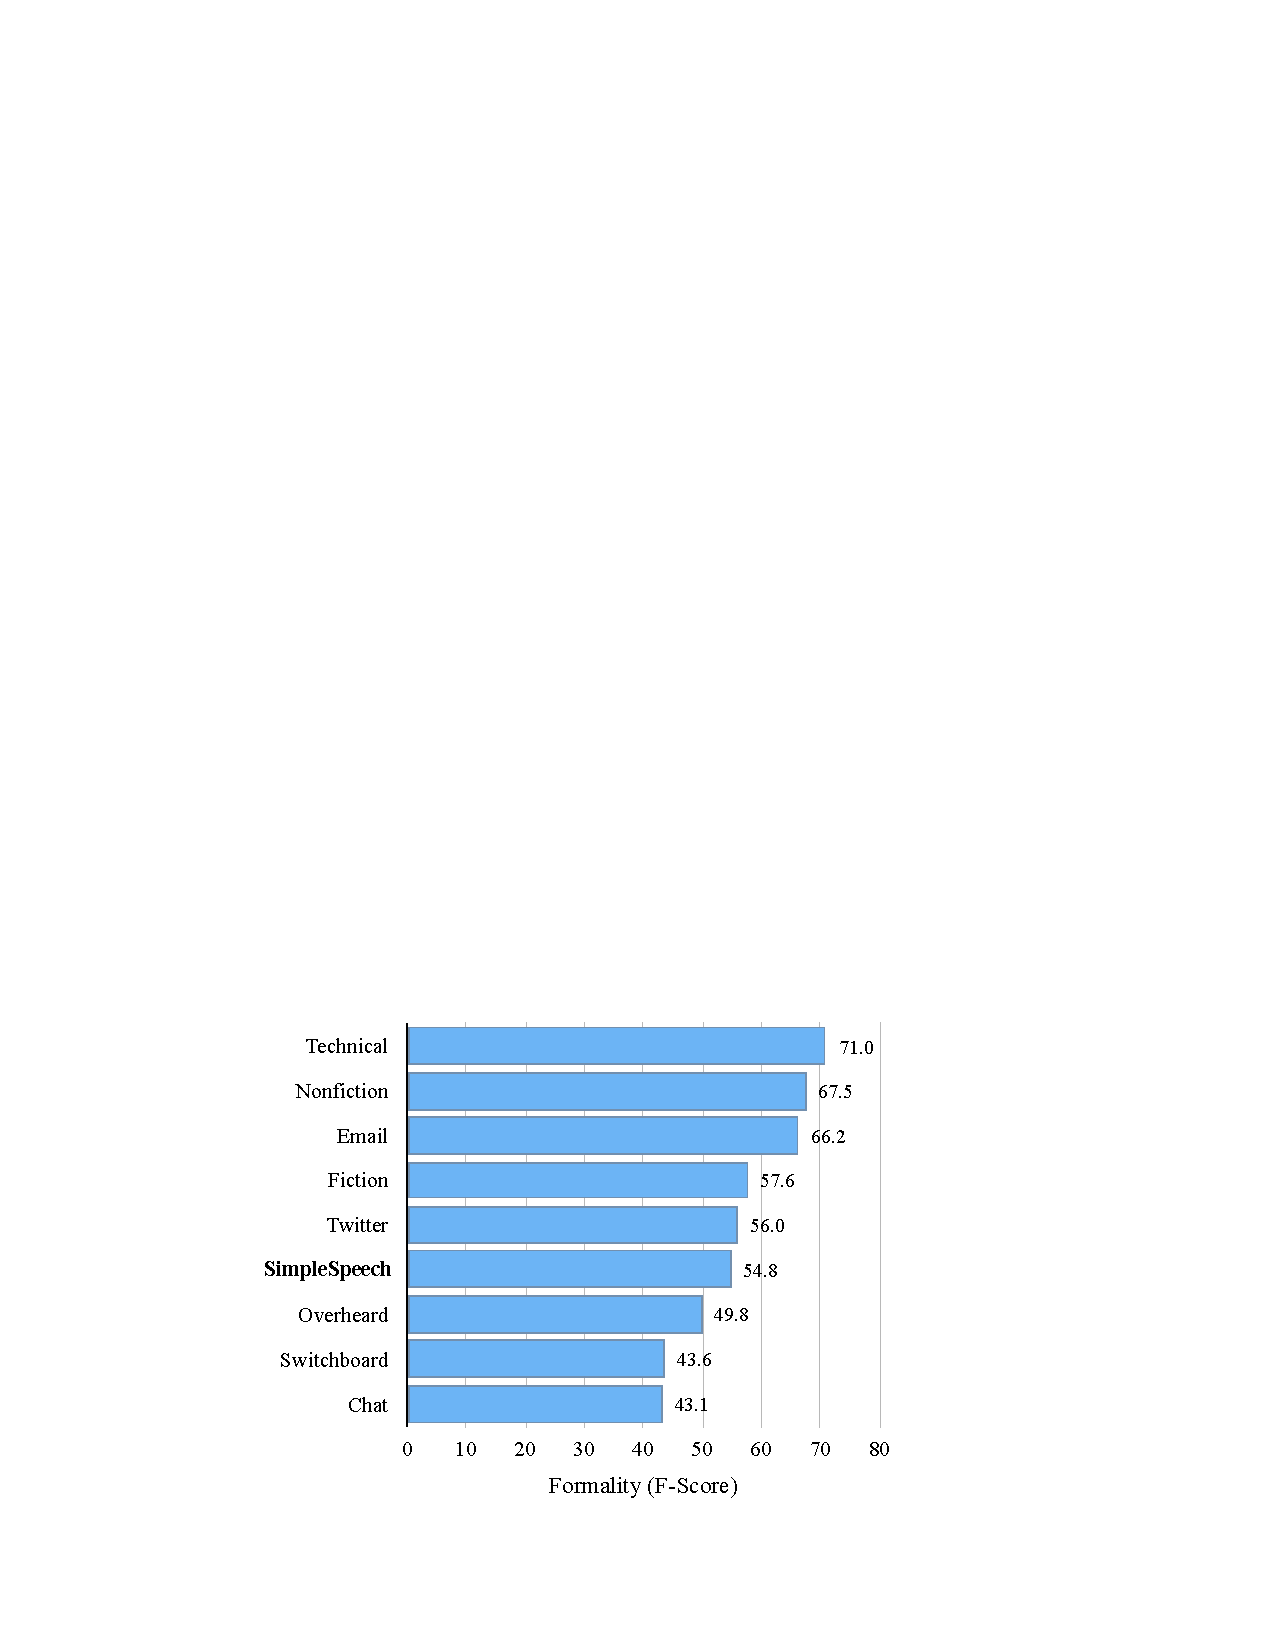
\includegraphics[width=\columnwidth,keepaspectratio]{figures/formality_comparison}
	\caption{The formality of corpora in different genre and media. The messages produced using SimpleSpeech during the quantitative study are intended to reflect general AAC discussion characteristics, and seem to be more formal than other spoken forms of communication but not as formal as email.}~\label{fig:formality}
\end{figure}

\emph{Speaker-audience relationship}. 
Since the F-score is inversely related to contextuality, it is reasonable that the chat and telephone corpora had the lowest F-scores because the participants knew each other and were conversing on a one-to-one basis. 
On the other hand, the written forms of communication (with the exception of email) were more formal because the audience was defined more loosely and not necessarily acquainted with the speaker.
AAC using SimpleSpeech was more closely related to the latter condition (as an online forum discussion), which probably contributed to its greater formality compared to the other spoken corpora.

\emph{Immediacy of communication}. 
The tendency to speak or write more contextually when the recipient replies immediately explains why the online chat text, though written, was more contextual and less formal than the oral corpora. 
It also justifies the fact that the email corpus was more formal than all of the other direct communication media.
Again, AAC falls toward the more formal end of this spectrum because there is little temporal proximity between the speaker and the audience.

\emph{Tendency toward verbosity}.
Media that pressured the creator to be brief or precise were more formal and less contextual.
For instance, writing technical documents requires the preferential use of nouns over pronouns to maximize clarity.
Twitter messages are, of course, limited to 140 characters, leading to a greater concentration of meaning that favors less contextual words.
For AAC, therefore, the ability to edit could influence the contextuality if discussion members were pressured to trim down their recordings. 
For our study, however, the participants were not affected by verbosity; though non-edited recordings had on average 10\% more words than edited ones, these edits were more concentrated on removing disfluencies than improving concision.

\section{Discussion}
In this study two forms of responding to pressure in a communication task were measured: the mental workload involved in completing the task and the degree of formality in the messages created in the task.
Using this information, we will evaluate the strengths and weaknesses of SimpleSpeech as a tool for enabling AAC as well as the viability of AAC in educational and collaborative contexts.

\subsection{Imbalance Between Speaker and Listener}
As Grudin notes, it is critical for collaborative software to spread the burden of usage equally on its constituent members. 
For instance, he cites email as a medium in which ``everyone generally shares the benefits and burdens equally'' \cite{grudin}. 
On the other hand, voice applications create inequality between speaker and listener since the former must expect that the latter will listen thoroughly and carefully to the message, a relatively slow task compared to reading.

However, the premise of SimpleSpeech is that the bias toward the speaker is reversed. 
ASR transcription can greatly facilitate the listener's task, as has already been demonstrated \cite{whittaker,vemuri}, bringing the workload down and closer to that of reading. 
Meanwhile, students who record messages could experience a \textit{greater} workload relative to writing because of the linearity of audio, which prevents them from correcting mistakes after the fact and thereby elevates the pressure to do well the first time.

SimpleSpeech was demonstrated to be a useful counterbalance in situations where the speaker's workload is elevated. 
In the qualitative study, some users noted the pressure ``to have organized thoughts'' and to ``sound composed more'' during recording, but that ``editing would make it nicer because you can go back and fix the mistakes'' ($P_2$).
Furthermore, the level of control was just right for most users: since they focused on deleting the disfluencies and pauses in their speech, the word-tokenized editor for the most part provided exactly the information needed to quickly delete undesirable sounds.
For the few users who did want to edit on a larger scale, the audio insertion feature was deemed helpful as well.

In the quantitative evaluation, we found strong evidence to support the use of SimpleSpeech, especially for students.
There was a significant decrease in task load on students when given the capability to edit, even in spite of the added time required to listen to the message and perform the editing.
The especially compelling factor is the Performance dimension, which decreased by 17\% in the Editing task. 
Several students also mentioned relief at the fact that the voice comments they were producing in the NE task would be anonymized; considering that most applications of AAC would not afford them this security, editing would become even more important to students' comfort level in voice communication.
On the other hand, teachers did not find SimpleSpeech as useful, probably because they already perceived their recordings as being of acceptable quality. 
One teacher reasoned that he was ``already used to hearing [his] own voice'' from lecturing, a medium where statements cannot be retracted as easily as with SimpleSpeech.
However, many teachers did use the editing tools, even though their workload levels were not significantly different with or without this opportunity.
This would indicate that the editing tools are a valuable option for producers to have, but users should not be obligated to use them.

\subsection{Editing and the Quality of Discussion}
Since even suggesting the use of editing tools potentially increased workload in the quantitative study, it is critical to the success of general-purpose AAC that the quality of discussion \emph{not} be driven up by a pressure to polish recordings.
Luckily, the formality of the discussions simulated in this study was not significantly affected by the stimulus recordings, indicating that for the most part, users are likely to adopt their own style for audio messages without being pressured by the discussion context.
Furthermore, for students this impetus toward quality is not as problematic, since they felt more relaxed rather than more stressed with editing functionality.
If discussion quality were driven up by artificial means, however, such as by grading students on the eloquence of their comments or evaluating employees on the basis of their online interactions, then individuals might gravitate toward ``safer'' modes of communication over which they feel more control (namely, text).
Proper acquaintance with audio editing capabilities is essential for AAC's survival under these pressures toward high-quality production.

\subsection{Implications for Formality in AAC}
AAC has the potential to greatly improve communication in educational, corporate, governmental, and personal contexts.
However, it is important that the social dynamics of AAC be taken into account in order to avoid unproductive, undesirable, or unwilling participation in collaborative environments.
For instance, discussion groups within an online course would be an ideal use of AAC using SimpleSpeech because students could send messages to a well-defined audience, thereby compensating for the additional formality imposed by the spatiotemporal distance between the participants. 
The editing tools would also drive students to produce better discussion input, increasing productivity and enhancing the learning experience.
On the other hand, enabling editing for personal communication, such as WhatsApp voice messages, would be detrimental to the desired informal speaking style of the platform.
Since the contextuality demanded by each situation is different, future audio-based collaboration platforms must consider the factors presented here and tailor their functionality accordingly.ß

\section{Conclusions}

SimpleSpeech's intuitive design alleviates the pressure associated with the linearity of audio because users have the capability to easily remove superfluous words, pauses, and sounds as well as insert new phrases, all after the fact.
Furthermore, we designed SimpleSpeech to clearly distinguish audio and text modalities, from the visual cues provided by the waveform to the quasi-modal interface for correcting transcription errors.
Students' use of these editing tools resulted in them feeling more comfortable producing comments than they were without SimpleSpeech functionality.
The true utility of this software, then, was to (at least partly) un-linearize audio, even making it more text-like.

Because studies of the linguistic and social characteristics of computer-mediated communication have been mostly limited to textual interactions, we also explored the formality and contextuality of AAC. 
Our finding that it was roughly in between spoken and written media is not discouraging \textit{per se}; however, the relatively formal characteristics of AAC must be taken into account before such a system is implemented in practice.
Nevertheless, we feel that the small-scale edits that users engaged in during this study are reassuring for potential applications of AAC.
Removing disfluencies and pauses allows users to feel comfortable with their recording while maintaining the spontaneity of thought in a spoken message.

The results of the qualitative study point to new directions for improving SimpleSpeech. 
For instance, on initial exposure to the application users initially tended to focus preferentially on the text instead of on the voice.
Slightly different visual layouts of the application, such as overlaying or juxtaposing the transcription on a more prominent waveform, could help users understand better that the text is a secondary tool.
Another possible feature could be automating certain edits, such as removing disfluencies and hesitations, to improve efficiency and edit quality even further.
Additionally, the findings in our quantitative study revealed promising trends concerning the benefits of AAC for online discussion, but may need a larger pool of test participants to attain statistical significance.

Our hope in developing SimpleSpeech is that asynchronous audio communication will gain greater usage in education and other collaborative settings. 
With the combination of ASR transcription for listeners and low-barrier editing tools for speakers, voice-based communication tools can engage students and improve the quality of collaboration on the Web.

\section{Acknowledgments}

Anonymized

% Balancing columns in a ref list is a bit of a pain because you
% either use a hack like flushend or balance, or manually insert
% a column break.  http://www.tex.ac.uk/cgi-bin/texfaq2html?label=balance
% multicols doesn't work because we're already in two-column mode,
% and flushend isn't awesome, so I choose balance.  See this
% for more info: http://cs.brown.edu/system/software/latex/doc/balance.pdf
%
% Note that in a perfect world balance wants to be in the first
% column of the last page.
%
% If balance doesn't work for you, you can remove that and
% hard-code a column break into the bbl file right before you
% submit:
%
% http://stackoverflow.com/questions/2149854/how-to-manually-equalize-columns-
% in-an-ieee-paper-if-using-bibtex
%
% Or, just remove \balance and give up on balancing the last page.
%
\balance{}

% REFERENCES FORMAT
% References must be the same font size as other body text.
\bibliographystyle{SIGCHI-Reference-Format}
\bibliography{sample}

\end{document}

%%% Local Variables:
%%% mode: latex
%%% TeX-master: t
%%% End:
